\section{Data description}
In order to build a system which would visualize the various sound points in and around a particular geographical location and also allow us to analyse the mismatches between the test and machine data, we need to have a dataset which has a diverse distribution of labeled sounds with spatial and temporal attributes. For which we have taken a dataset containing a training subset (13538 recordings from 35 sensors), validation subset (4308 recordings from 9 sensors), and a test subset (669 recordings from 48 sensors). Each recording has been annotated using a set of 23 “sound tags” like “engine presence, machinery presence, non-machinery-impact presence, dog-barking-whining presence, music presence etc.”  ~\cite{4}.

	\begin{figure}[h!]
	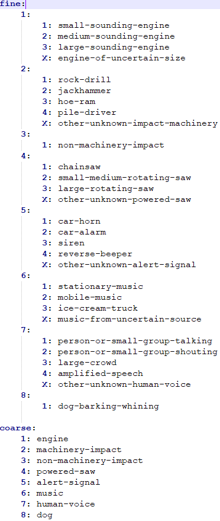
\includegraphics[width=6cm]{figure5}
	\caption{A snapshot of the dataset labels}
\end{figure}

fig 1 shows all the fine level and course level classes. The course level lists down all the different catagories of  sound samples that are captured, whereas fine level describes the all the sub-classes in these main classes. For example the group Engine has small-sounding-engine, medium-sounding-engine, large-sounding-engine as the fine-level classes.

The training, validation, and test subsets of the annotation data are contained in annotations.csv (see Figure 1). Each row in the file represents one multi-label annotation of a recording—it might be a single citizen science volunteer's annotation, a single SONYC team member's annotation, or the SONYC team's agreed-upon ground truth (for more information, see the annotator id in column description).The audio files used were recorded using the SONYC acoustic sensor network for monitoring urban noise pollution. In New York City, over 60 distinct sensors have been placed accumulating the equivalent of more than 50 years of audio data, of which a small fraction is used. The data is sampled by picking the closest neighbors based on VGGish qualities of recordings with recognized classes of interest. All of the recordings are 10 seconds long and were made with the same microphones and gain settings. 

The sensors in the test set will not disjoint from the training and validation subsets, but the test recordings are displaced in time, occurring after any of the recordings in the training and validation subset. We plan to use the test data to find out the aggregate of mismatch by using a Multi Label classification Machine Learning Model like support vector machines and artificial neural networks.

In our work we will utilize the latitude and longitude columns to spatially locate the sound origin, the year, week, day, hour columns to precisely point the time and the category column which contain engine, machinery-impact, non-machinery-impact, powered-saw etc.to get the sound type to analyze and visualize the data.
	\begin{figure}[h!]
		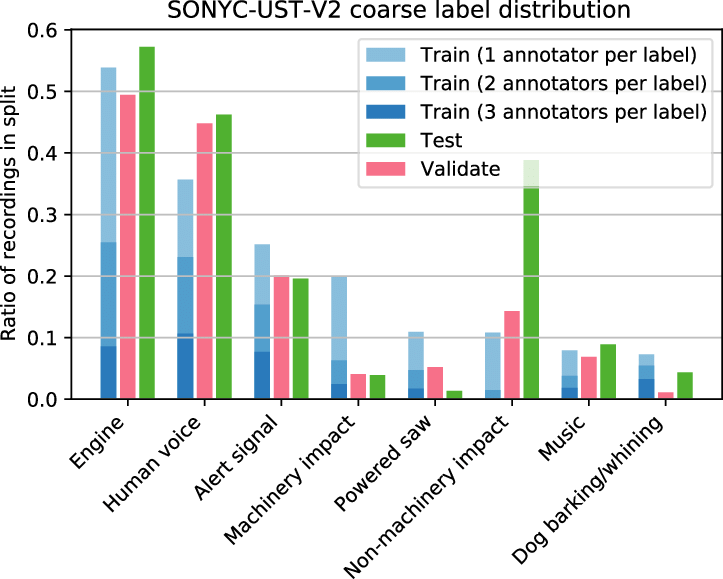
\includegraphics[width=9cm]{figure1}
		\caption{Distribution of various sound tags in test, train, validate sets of dataset}
	\end{figure}
	


	
	
	
	

	
	